%%%%%%%%%%%%%%%%%%%%%%%%%%%%%%%%%%%%%%%%%%%%%%%%%%%%%%%%%%%%%%%%%%%%%%%%%%%%%%%
%%  claude-giga-lens --- TECHNICAL REPORT (scaffold + settled sections).
%%
%%  Correlated-Noise Likelihoods and Next-Generation Inference for Strong
%%  Gravitational Lens Modeling.
%%
%%  Settled sections (final prose, all numbers cited to data/*.json + CAMPAIGN.md):
%%    1 Intro, 2 Data & targets, 3 Methods I (correlated likelihood),
%%    4 Methods II (zoo + protocol), 5 Mock validation, 7 Sampler benchmark,
%%    9 Discussion, 10 Reproducibility, App A/C/D (B partial).
%%  Gated sections carry \todo{} placeholders (see "List of Open (Gated) Items"):
%%    6 Real-data cross-scale (P1c), 8 CGL recipe end-to-end + Euclid Q1 (P3),
%%    T2/T3 rows of the benchmark (P2c).
%%
%%  Single-column article + shared preamble reproductions/tech-report.sty
%%  (natbib + bibtex). Builds with vanilla TeX Live (>= 2022): make pdf.
%%%%%%%%%%%%%%%%%%%%%%%%%%%%%%%%%%%%%%%%%%%%%%%%%%%%%%%%%%%%%%%%%%%%%%%%%%%%%%%
\documentclass[11pt,letterpaper]{article}
\usepackage{../../tech-report}
\usepackage{lmodern}   % scalable Type1 fonts (microtype auto-expansion needs them)

% --- Lensing / method math macros -------------------------------------------
\newcommand{\thetaE}{\ensuremath{\theta_{\mathrm{E}}}}
\newcommand{\gammaEPL}{\ensuremath{\gamma}}
\newcommand{\gext}{\ensuremath{\gamma_{\mathrm{ext}}}}
\newcommand{\gextone}{\ensuremath{\gamma_{1}}}
\newcommand{\gexttwo}{\ensuremath{\gamma_{2}}}
\newcommand{\eone}{\ensuremath{e_{1}}}
\newcommand{\etwo}{\ensuremath{e_{2}}}
\newcommand{\Rhat}{\ensuremath{\hat{R}}}
\newcommand{\ESS}{\textrm{ESS}}
\newcommand{\eop}{\ensuremath{e_{\mathrm{op}}}}
\newcommand{\Neff}{\ensuremath{N_{\mathrm{eff}}}}
\newcommand{\foundry}{DESI--165.4754$-$06.0423}
\newcommand{\gigalens}{\textsc{GIGA-Lens}}
\newcommand{\gigalenstwo}{\textsc{GIGA-Lens\,2.0}}
\newcommand{\lenstronomy}{\textsc{lenstronomy}}
\newcommand{\photutils}{\textsc{photutils}}
\newcommand{\herculens}{\textsc{herculens}}
\newcommand{\nautilus}{\textsc{nautilus}}
\newcommand{\flowmc}{\textsc{flowMC}}
\newcommand{\blackjax}{\textsc{BlackJAX}}
\newcommand{\coolest}{\textsc{COOLEST}}
\newcommand{\art}[1]{\footnote{Source artifact: \texttt{#1}.}}
\newcommand{\dfile}[1]{\texttt{#1}}

% --- \todo{} macro: colored, counted, and collected in a "List of Open Items"
\makeatletter
\newcounter{todocnt}
\newcommand{\todo}[1]{%
  \refstepcounter{todocnt}%
  {\color{red}\bfseries[\,TODO~\thetodocnt:\ #1\,]}%
  \addcontentsline{tdo}{todo}{\protect\numberline{\thetodocnt}#1}%
}
\newcommand*{\l@todo}[2]{%
  \par\noindent\hangindent2.2em\hangafter1
  {\color{red}\bfseries\@dottedtocline{1}{0em}{2.0em}{#1}{#2}}}
\newcommand{\listoftodos}{%
  \section*{List of Open (Gated) Items}%
  \addcontentsline{toc}{section}{List of Open (Gated) Items}%
  {\small\@starttoc{tdo}}}
\makeatother

% --- A framed placeholder for a figure that is gated on a future result -----
\newcommand{\gatedfigure}[3]{% #1=label #2=caption #3=todo text
  \begin{figure}[ht]\centering
  \setlength{\fboxsep}{10pt}%
  \fbox{\parbox{0.86\textwidth}{\centering
    \textit{Figure placeholder --- content gated on a pending result.}\par
    \smallskip {\color{red}\bfseries[\,gated: see open item below\,]}}}%
  \caption{#2}
  \label{#1}
  \end{figure}%
  \par\noindent\todo{#3}\par}

\title{Correlated-Noise Likelihoods and Next-Generation Inference
       for Strong Gravitational Lens Modeling\thanks{All work reported
       here --- code, experiments, analysis, and text --- was performed
       by Claude Code (Anthropic), guided by Greg Benson. This document
       is a technical report: its two gated results sections
       (\S\ref{sec:realdata}, \S\ref{sec:recipe}) carry colored
       open-item placeholders to be filled when the P1c and P3 runs
       complete.}}
\author{Greg Benson\thanks{Department of Computer Science, University of
        San Francisco, CA 94117, USA; \texttt{greg.benson@gmail.com}.} \and
        Xiaosheng Huang\thanks{Department of Physics \& Astronomy,
        University of San Francisco, CA 94117; and Physics Division,
        Lawrence Berkeley National Laboratory, CA 94720.}}
\date{July 2026\\[3pt]{\small\texttt{commit:~b004927}}}

\begin{document}
\maketitle
\subtitle{Technical report: P1/P2 methods settled; real-data verdict (P1c),
A100 sampler matrix (P2c), and end-to-end recipe (P3) gated}

\begin{abstract}
Drizzled space-based imaging carries strongly correlated pixel noise that
the per-pixel diagonal Gaussian likelihood --- the statistical core of every
fast GPU lens modeling code, including \gigalens\ \citep{gu2022gigalens} and
its recent multi-node successor \gigalenstwo\ \citep{huang2026gigalens2} ---
simply ignores. On the {\it HST}/WFC3-IR system \foundry\ this omission
produces a scale-dependent power-law slope \gammaEPL\ (1.29 binned, 1.43
native, a 2.585 artifact on the upsampled fine product) and a two-basin
\gammaEPL\ posterior \citep{huang2025foundry1}. We report a scaffold and the
settled methodology of a campaign that changes what \gigalenstwo\ leaves
unchanged: the likelihood and the sampler. We build a drizzle-anchored
correlated-noise likelihood ($C=D^{1/2}KD^{1/2}$, convolutional whitening,
operator-norm whiteness gate $\eop\le0.02$) integrated with a generalized
ridge marginalization of the linear source amplitudes and its Gaussian
evidence (Occam) term; it reduces {\it exactly} to the validated diagonal
stack ($|\Delta\log L|=0$ at machine precision), matches a dense-covariance
Cholesky reference to $<3\times10^{-9}$~nat, and reproduces the diagonal
miscalibration in miniature on drizzle mocks (median $|z(\gammaEPL)|=5.84$).
Under a two-stage preconditioned-HMC recipe (itself a finding: it lowers
\Rhat\ from $2.11$ to $1.003$), the correlated likelihood is calibrated on
mocks (depth-controlled bias $|\bar z(\gammaEPL)|<0.5$ at every scale;
simulation-based-calibration rank tests pass on healthy fits) and is found to
be {\it conservative, not biased} ($\sigma_{\rm fine}/\sigma_{\rm
native}=2.45$, a characterized information cost of near-singular drizzle
covariances). Independently, we deliver the first systematic sampler and
multimodality benchmark on strong-lens posteriors: nine contenders across a
$19$-target, four-tier ``posterior zoo,'' under a pre-registered,
budget-matched, tuning-frozen protocol ($370$ evaluation cells). The headline
is two-sided: \nautilus\ dominates sampling efficiency ($2.6$--$307\times$
ESS/gradient) but is disqualified on the real-lens ill-conditioned
marginalization regime; no gradient method beats the \gigalens\ baseline at
budget parity; parallel-tempered HMC is the most reliable until-converged; and
\flowmc\ fails structurally on these geometries. The real-data cross-scale
unification verdict (P1c), the A100 sampler matrix on the hardest targets
(P2c), and the end-to-end recipe on \foundry\ plus Euclid Q1 (P3) are
pre-registered and gated; their section frames and hypotheses are stated
here. Every quantitative claim is traced to a JSON artifact and a gate record
in \texttt{CAMPAIGN.md}.
\end{abstract}

\listoftodos
\medskip

%%%%%%%%%%%%%%%%%%%%%%%%%%%%%%%%%%%%%%%%%%%%%%%%%%%%%%%%%%%%%%%%%%%%%%%%%%%%%%%
\section{Introduction}
\label{sec:intro}
%%%%%%%%%%%%%%%%%%%%%%%%%%%%%%%%%%%%%%%%%%%%%%%%%%%%%%%%%%%%%%%%%%%%%%%%%%%%%%%

Galaxy-scale strong lensing constrains the inner density profiles of massive
galaxies and, through time-delay cosmography, the Hubble constant
\citep{treu2010annurev,tdcosmo4}. The precision of these constraints is now
limited less by data volume than by modeling systematics. The Time-Delay Lens
Modeling Challenge \citep{tdlmc2018,tdlmc2020results} established blind,
truth-known benchmarking as the discipline's standard for exposing such
systematics; but since its first round the community has produced few
successors of comparable rigor, even as the modeling codes have accelerated
by orders of magnitude. The recent code-comparison study of
\citet{etherington2024codecomparison} quantifies the resulting exposure:
holding the data fixed and varying only the source model and modeling method
shifts the recovered logarithmic density slope \gammaEPL\ by $\sim$$2\%$ ---
a systematic that rivals or exceeds the statistical error bars quoted on
individual systems. That same study flags two ingredients as under-addressed
in fast lens modeling: correlated image noise (their motivation cites the
strongly correlated noise of resampled JWST imaging) and honest posterior
multimodality. Both remain open: no flagship lens-modeling paper implements a
correlated-noise likelihood in a fast GPU code, and none uses flow-assisted or
transport-preconditioned samplers, where nested sampling
\citep{lange2023nautilus} otherwise dominates.

\gigalens\ \citep{gu2022gigalens} pioneered GPU-accelerated Bayesian lens
modeling with a multi-start MAP $\to$ SVI $\to$ preconditioned-HMC recipe in
JAX, and has been applied to spectroscopically confirmed systems
\citep{cikota2023einsteincross,sheu2024carousel} and to the DESI Strong Lens
Foundry \citep{huang2025foundry1}. Its recent successor \gigalenstwo\
\citep{huang2026gigalens2} distributes exactly this recipe to $128$ nodes /
$512$ A100 GPUs on NERSC Perlmutter, achieving --- for the first time on a
real system --- $\Rhat<1.01$ on all $38$ parameters of a DESI lens in
$\sim$$25$~minutes on eight nodes. Crucially, that work {\it scales the
computation while leaving the statistical model untouched}: the likelihood
remains the per-pixel diagonal Gaussian of \citet{gu2022gigalens}, source
amplitudes are solved (not marginalized) by linear inversion, and a single
Gaussian SVI surrogate seeds HMC, presuming a unimodal posterior. As we detail
in the campaign's positioning analysis,\art{research/notes/gigalens2-positioning.md}
\gigalenstwo\ has zero overlap with the two axes this campaign advances: it
introduces no noise covariance, no analytic marginalization or Occam factor,
and no tempering, nested sampling, or normalizing flows. Faster inference of
a mis-specified likelihood converges faster to the wrong posterior; our
contribution is to fix what is being scaled.

The precipitating evidence is the Foundry-I reproduction of \foundry\
\citep{huang2025foundry1}, which closed with two explicit open items. First,
the drizzled {\it HST} products have strongly correlated pixel noise ---
measured lag-1 correlation $\rho(1)=0.795$ on the $0\farcs04$ fine product,
$0.52$ at native scale, with an effective independent-pixel fraction
$\Neff/N\approx0.017$ --- that the diagonal likelihood ignores, producing a
{\it scale-dependent} slope (1.29 binned / 1.43 native / a 2.585 artifact on
the fine product) and a genuinely disconnected two-basin \gammaEPL\ posterior
on the binned product (45 of 48 chains in the low basin, 3 in the steep basin,
zero inter-basin migrations). Second, HMC on such degenerate and multimodal
lens posteriors is the binding computational constraint. This campaign
attacks both.

We state two contributions.
\begin{enumerate}
\item {\bf A correlated-noise (drizzle) likelihood with generalized ridge
marginalization.} We model the pixel covariance as
$C=D^{1/2}KD^{1/2}$ with $D$ the existing heteroscedastic diagonal and $K$ a
stationary, drizzle-anchored correlation kernel fit on model-subtracted
residuals; we whiten it by a truncated convolutional operator gated on its
operator-norm flatness; and we integrate the whitening into an analytic
ridge-marginalization of the linear (shapelet) source amplitudes that carries
the Gaussian-evidence (Occam) term that the plain linear solve omits. The
machinery reduces {\it exactly} to the validated diagonal stack in the
white-noise limit, is validated against a dense-covariance Cholesky reference,
is calibrated on drizzle mocks with known truth, and is tested --- in the
gated \S\ref{sec:realdata} --- against a pre-registered cross-scale
unification hypothesis on the real system.
\item {\bf The first systematic sampler / multimodality benchmark on
strong-lens posteriors.} We assemble a $19$-target ``posterior zoo'' spanning
analytic synthetic targets, twelve \citet{gu2022gigalens} mocks, the
$46$-dimensional condition-number-$10^{14}$ marginalized real posterior, and
the $74$-dimensional bimodal real posterior, and benchmark nine samplers ---
including a normalizing-flow / neutral-transport recipe --- under a
budget-matched, tuning-honest, pre-registered protocol.
\end{enumerate}

This report is the {\bf scaffold and settled methodology} of the campaign. The
correlated-likelihood construction and validation (\S\ref{sec:methods1},
\S\ref{sec:mocks}), the benchmark protocol and its phoenix-scale results
(\S\ref{sec:methods2}, \S\ref{sec:benchmark}), and the reproducibility
substrate (\S\ref{sec:repro}) are final. The real-data cross-scale verdict
(\S\ref{sec:realdata}; P1c), the A100 sampler matrix on the hardest targets
(\S\ref{sec:benchmark}, tiers T2/T3; P2c), and the end-to-end recipe on
\foundry\ and Euclid Q1 \citep{euclidq1_slde_2025} (\S\ref{sec:recipe}; P3) are
gated on runs not yet complete; their frames, pre-registered hypotheses, and
figure slots are laid out so that filling them requires no re-design. The
campaign follows the repository's retraction culture: goalposts (the verbatim
thresholds of Table~\ref{tab:thresholds}) were frozen before any science ran,
and every number below is traced to a JSON artifact and a dated gate record in
\texttt{CAMPAIGN.md}.

%%%%%%%%%%%%%%%%%%%%%%%%%%%%%%%%%%%%%%%%%%%%%%%%%%%%%%%%%%%%%%%%%%%%%%%%%%%%%%%
\section{Data and Targets}
\label{sec:data}
%%%%%%%%%%%%%%%%%%%%%%%%%%%%%%%%%%%%%%%%%%%%%%%%%%%%%%%%%%%%%%%%%%%%%%%%%%%%%%%

\subsection{The real system and its three drizzle products}

We model \foundry, observed with {\it HST}/WFC3-IR in F140W under program
GO--15867 (public via MAST DOI 10.17909/hx0v-9260) and reduced by
\citet{huang2025foundry1} into three data products at different pixel scales,
each with its own empirical PSF and heteroscedastic error map
(Table~\ref{tab:products}). The scales differ by resampling: the native
$0\farcs128$ product (\dfile{v2d}, $80^2$~px) is the pipeline drizzle at its
true plate scale, the fine product (\dfile{v3}, $0\farcs04$, $260^2$~px) is a
MAST HAP fine-skycell mosaic of the same exposures, and the binned product
(\dfile{v3b}, $0\farcs08$, $130^2$~px) is a $2\times2$ rebuild of the fine
mosaic. Because drizzle \citep{fruchterhook2002drizzle} distributes each input
pixel's flux over an output footprint, the resampled products carry noise that
is correlated on the drizzle-kernel scale
(\S\ref{sec:methods1}).\art{data/noise\_kernel\_report.json} The
model-subtracted residual autocorrelation confirms this directly: the along-axis
lag-1 correlation is $\rho(1)=0.815$ on the fine product, $0.615$ binned, and
$0.305$ native.\footnote{These are the along-axis correlations of the
detrended, model-subtracted residual measured for the kernel fit
(\dfile{data/noise\_kernel\_report.json}); the $\rho(1)=0.795$/$0.52$
fine/native figures quoted in the introduction and in \citet{huang2025foundry1}
are the isotropic sky-autocorrelation values of the raw product. Both express
the same fact: the fine grid is heavily oversampled relative to its resolution
element.}

\begin{table}[ht]
\centering
\caption{The three drizzle products of \foundry\ and their measured noise
correlation. Kept-pixel counts are after mask erosion by the whitening stencil
(\S\ref{sec:methods1}); $\rho(1)$ is the along-axis lag-1 correlation of the
model-subtracted residual.}
\label{tab:products}
\begin{tabular}{lccccc}
\toprule
tag & scale ($''$) & grid & $\rho(1)$ & kept px & role \\
\midrule
\dfile{v3}  (fine)   & 0.04  & $260^2$ & 0.815 & 66{,}752 & most correlated; artifact host \\
\dfile{v3b} (binned) & 0.08  & $130^2$ & 0.615 & 16{,}653 & bimodal-\gammaEPL\ host \\
\dfile{v2d} (native) & 0.128 & $80^2$  & 0.305 &  5{,}865 & diagonal-trustworthy anchor \\
\bottomrule
\end{tabular}
\par\smallskip
{\footnotesize\textit{Note.} Effective independent-pixel fraction
$\Neff/N\approx0.017$; a $2\times2$ fine-pixel block is $\sim$$78\%$
internally correlated. The native product is where the diagonal likelihood is
least wrong and anchors the cross-scale comparison (\S\ref{sec:realdata}).}
\end{table}

\subsection{The drizzle-mock generator}
\label{sec:mocks-gen}

Calibration with known truth requires mocks whose noise correlation is
generated by the {\it same} drizzle operator that the likelihood models. Our
generator (\dfile{05\_gen\_drizzle\_mocks.py}) renders a noiseless lensed
image on the fine grid, applies the analytic $3\times3$ separable tent
convolution induced by the $3$-frame drizzle, and adds correlated noise with
the exact analytic covariance of each product. Machine-precision self-consistency
is enforced: the noiseless render agrees with the drizzle operator to a worst
deviation of $2.1\times10^{-12}\sigma$ over $8$ mock trios, far inside the
$0.05\sigma$ gate.\art{data/mocks\_report.json}

One deviation is preserved deliberately as a real-data caveat.\art{data/mocks\_report\_3frame.json}
A na\"ive $3$-dither Latin stack $\{(0,0),(1,2),(2,1)\}$ is {\it provably
shift-variant} --- no single effective convolutional PSF exists, and the
render check fails at $2.1$--$26.7\sigma$. The mocks therefore use all nine
dither phases, for which the effective PSF is exactly the separable $3\times3$
tent. The real \dfile{v3} skycell (\texttt{NDRIZIM}$=3$) is likewise
shift-variant: its ``effective PSF'' is an approximation, a genuine limitation
of stationary-kernel modeling on real drizzle that we flag rather than hide.

\subsection{The posterior zoo}
\label{sec:zoo-data}

For the sampler benchmark (\S\ref{sec:methods2}) we freeze a four-tier
``posterior zoo'' of $19$ targets that exercises distinct pathologies:
analytic synthetic targets with known evidence and modes (T0), the twelve
\citet{gu2022gigalens} mock systems (T1), the $46$-dimensional
marginalized real posterior of \foundry\ at condition number $\sim$$10^{14}$
(T2), and its $74$-dimensional genuinely bimodal binned posterior (T3). The
full specification is Appendix~\ref{app:zoo}. The Euclid Q1 targets (T4)
\citep{euclidq1_slde_2025} are a stub for the gated end-to-end phase
(\S\ref{sec:recipe}).

%%%%%%%%%%%%%%%%%%%%%%%%%%%%%%%%%%%%%%%%%%%%%%%%%%%%%%%%%%%%%%%%%%%%%%%%%%%%%%%
\section{Methods I --- The Correlated-Noise Likelihood}
\label{sec:methods1}
%%%%%%%%%%%%%%%%%%%%%%%%%%%%%%%%%%%%%%%%%%%%%%%%%%%%%%%%%%%%%%%%%%%%%%%%%%%%%%%

\subsection{Covariance model and drizzle anchor}

We factor the pixel covariance as
\begin{equation}
  C \;=\; D^{1/2}\,K\,D^{1/2},
  \label{eq:cov}
\end{equation}
where $D=\mathrm{diag}(\sigma_i^2)$ is the existing heteroscedastic error map
(masks retained as $\sigma\to10^{10}$) and $K$ is a stationary correlation
matrix, fixed per product, generated by a kernel $\rho(\Delta)$ fit on the
{\it model-subtracted} residual autocorrelation (a guard-enforced requirement,
so diffuse lens flux cannot bias the calibration). The kernel is anchored on
the analytic drizzle correlation: for a square pixel of drizzle radius
$r=3.2075$ fine pixels the closed-form along-axis lag-1 correlation is
$t(1)=0.76805$, matched by the enumerated drizzle operator to
$0.76799$.\art{data/noise\_kernel\_report.json}

\paragraph{Kernel family (deviation from the naive two-parameter plan).}
The pre-registered plan proposed a single-Gaussian family
$\rho=(1-w)\delta + w\,[\rho_{\rm drz}\!\circledast G(\sigma_e)]$. This family
cannot pass the $\max|\rho_{\rm fit}-\rho_{\rm meas}|\le0.05$ gate on any
product (best residuals $0.090$/$0.311$/$0.166$ for
\dfile{v2d}/\dfile{v3}/\dfile{v3b}); the residuals carry a medium-scale
correlated pedestal, an anisotropic core, and, on \dfile{v2d}, column stripes.
We adopt the minimal positive-semidefinite-by-construction extension --- a
two-component bivariate form,
\begin{equation}
  \rho \;=\; (1-w_d-w_b)\,\delta
        \;+\; w_d\,\bigl[\rho_{\rm drz}\!\circledast G_2(\sigma_{ey},\sigma_{ex},c_e)\bigr]
        \;+\; w_b\,G_2(\sigma_{by},\sigma_{bx},c_b),
  \label{eq:kernel}
\end{equation}
whose PSD is a non-negative sum of a floor, the drizzle-anchored component, and
a broad bivariate-Gaussian pedestal. It passes on all three products
($\max|\rho_{\rm fit}-\rho_{\rm meas}|=0.0448$/$0.0270$/$0.0326$), with the
single-family failure numbers preserved on
record.\art{data/noise\_kernel\_report.json} An independent cross-check
validates the block-sum relation between scales: the binned kernel predicted
from the fitted fine kernel agrees with the binned kernel measured on the
block-summed fine residual to $0.031$ (gate $0.05$), confirming that our
kernels commute correctly with $2\times2$ binning; the product-level
disagreement ($0.0595$, informational) is the known non-commutation of the
\photutils\ background detrend with binning.

\subsection{Convolutional whitening}
\label{sec:whiten}

We whiten by a truncated convolution $h=\mathcal{F}^{-1}[S^{-1/2}]$, where
$S(\omega)$ is the kernel PSD, regularized by a spectrum floor
$s_{\rm floor}=0.05$ (the critical conservative regularizer: the true
fine-grid covariance is near rank-deficient), truncated to a $(2M+1)^2$ stencil
and Gauss--Newton refined. The operator is accepted only if its operator-norm
whiteness gate
\begin{equation}
  \eop \;=\; \max_\omega\bigl|\,S(\omega)\,|\hat h_M(\omega)|^2 - 1\,\bigr| \;\le\; 0.02
  \label{eq:eop}
\end{equation}
is met, {\it and} a Monte-Carlo whiteness check gives unit variance
($\mathrm{Var}(u)\in1\pm0.02$) and lag-$\le$3 off-diagonal correlation below
$0.01$. Masks are handled by a {\it whiten-then-drop} rule: we keep only
whitened pixels whose stencil avoids masks and the border (a
\texttt{binary\_erosion}), which is statistically exact. Table~\ref{tab:whiten}
summarizes the accepted whiteners. Two construction fixes were required in P1a:
kernels are stored analytically out to half-width $64$ to suppress truncation
ringing, and the spectrum floor is {\it adaptive} (a hard $0.05$ floor on an
already-PSD kernel biases $\mathrm{Var}(u)$ to $0.981$ and fails the gate).

\begin{table}[ht]
\centering
\caption{Accepted whiteners. $\eop$ is the operator-norm whiteness residual
(gate $\le0.02$); MC $\mathrm{Var}(u)$ and worst lag-$\le3$ off-diagonal from
$500$--$2000$ draws (gates $1\pm0.02$, $<0.01$). Pixel loss is mask/border
erosion by the $(2M{+}1)^2$ stencil.}
\label{tab:whiten}
\begin{tabular}{lccccc}
\toprule
product & $M$ & $\eop$ & $\mathrm{Var}(u)$ & worst off-diag & kept / eroded \\
\midrule
\dfile{v2d} (native, strict)   & 14 & 0.0177 & 1.004 & 0.0075 & 5{,}865\,/\,487 \\
\dfile{v3}  (fine)             & 20 & 0.0160 & 1.000 & 0.0003 & 66{,}752\,/\,37{,}519 \\
\dfile{v3b} (binned)           & 10 & 0.0124 & 0.999 & 0.0012 & 16{,}653\,/\,9{,}273 \\
\dfile{v2d\_relaxed} (native)  & 10 & 0.0312 & 1.001 & 0.0029 & 5{,}865\,/\,1{,}466 \\
\bottomrule
\end{tabular}
\par\smallskip
{\footnotesize\textit{Note.} The strict \dfile{v2d} whitener erodes to only
$487$ kept pixels ($91.7\%$ loss from the $29^2$ stencil at native scale). A
relaxed whitener ($\eop\le0.05$, $M{=}10$, $1466$ kept $=3.0\times$ strict) was
built as a pre-registered evidence-driven exception and adopted after mock
calibration held (\S\ref{sec:mocks}). Source:
\dfile{data/whitener\_report.json}.}
\end{table}

\subsection{Generalized ridge marginalization}
\label{sec:marg}

The $28$ shapelet source amplitudes are linear parameters; we marginalize them
analytically using their Gaussian priors as a Tikhonov ridge, generalizing the
diagonal-likelihood marginalization of \citet{huang2025foundry1} to the
whitened residual. Writing $\tilde X = W_e[\,D^{-1/2}\circledast h\,]X$ for the
whitened, PSF-convolved unit-amplitude design matrix ($W_e$ the keep-mask,
$\circledast h$ the whitening convolution) and $\tilde R$ for the whitened
residual after the deterministic components,
\begin{align}
  A &= \tilde X^{\!\top}\tilde X + \Lambda, &
  b &= \tilde X^{\!\top}\tilde R, &
  a^{\star} &= A^{-1}b, \label{eq:normaleq}\\
  \log L &= -\tfrac12\|\tilde R\|^2 + \tfrac12\,b^{\!\top}a^{\star}
            - \tfrac12\log\det A + \mathrm{const}, \label{eq:logl}
\end{align}
with $\Lambda_{ii}=(i+1)/25$ the prior precision (so $A\succ0$ and the solve is
Cholesky, never a pseudo-inverse), and $-\tfrac12\log\det A$ the
Gaussian-evidence (Occam) term. The additive constant absorbs
$-\tfrac12\log\det C$, which is $\theta$-independent (the kernels are fixed) and
therefore dropped for sampling but {\it stored}: cross-whitener evidence
comparisons must add it back, and the exact-versus-Szeg\H{o} constant gap is
$+27.30$ (\dfile{v2d}) and $+179.21$ (\dfile{v3b}) nat.\art{data/exact\_ref\_report.json}

\subsection{Exact-reference validation and the grouped-convolution fix}
\label{sec:exactref}

Two independent references certify the implementation. First, the {\it
diagonal limit}: with $C=D$ the whitened functional
(\ref{eq:normaleq})--(\ref{eq:logl}) must reduce {\it exactly} to the validated
diagonal stack. It does, to $|\Delta\log L|=0$ at machine precision across four
test points, and the whole marginalized log-posterior and its gradient
reproduce the Foundry-I \texttt{\_hmc\_lib\_marg} core to
$|\Delta\log p|=0$ and relative gradient $L_2 = 7\times10^{-17}$
(Appendix~\ref{app:parity}).\art{data/parity\_report.json} Second, the {\it
dense-covariance} reference: the convolution-whitened $\log L$ is compared
against a CPU float-64 dense-$C$ Cholesky on the kept pixels at $20$ prior
draws. The worst $|\Delta\log L|$ is $2.79\times10^{-9}$~nat (\dfile{v2d}) and
$6.26\times10^{-7}$~nat (\dfile{v3b}), both far inside the $0.1$-nat gate; on
the $260^2$ fine grid an FFT-preconditioned conjugate-gradient solve
(relative residual $10^{-8}$, $131$ iterations) reproduces the exact GLS
quadratic form.\art{data/exact\_ref\_report.json} We stress the gate's
semantics: it certifies {\it implementation-exactness} of the whitened
functional $C^{-1}:=G_e^{\!\top}G_e$; physical-$C$ misspecification is bounded
separately by $\eop$ (Eq.~\ref{eq:eop}), since exact-GLS equivalence at
individual prior draws is mathematically unattainable under any finite floor.

The batched gradient exposed a genuine stack defect
(\S\ref{sec:repro}, \#7): a \texttt{vmap} over chains of $28$ per-column
convolutional whitening operations {\it livelocks} the XLA compiler (100\% CPU,
GPU idle, $>$20~min), which disabling priority-fusion alone does not cure.
Collapsing the $28$ per-column convolutions into a single depthwise / grouped
convolution makes the batched gradient compile in $13.8$~s and leaves the
log-posterior bit-identical. The whitened correlated gradient then costs
$\le1.6\times$ the diagonal one ($40$/$85$~ms versus $25$/$55$~ms on an L4),
so the campaign runs at diagonal-comparable throughput.

%%%%%%%%%%%%%%%%%%%%%%%%%%%%%%%%%%%%%%%%%%%%%%%%%%%%%%%%%%%%%%%%%%%%%%%%%%%%%%%
\section{Methods II --- The Posterior Zoo and Benchmark Protocol}
\label{sec:methods2}
%%%%%%%%%%%%%%%%%%%%%%%%%%%%%%%%%%%%%%%%%%%%%%%%%%%%%%%%%%%%%%%%%%%%%%%%%%%%%%%

\subsection{The \texttt{LensPosterior} interface}

Every zoo target exposes a single frozen, jitted target through a
\texttt{LensPosterior} dataclass. Its defining feature is a {\it
\texttt{log\_prior} / \texttt{log\_like} split in $z$-space}, which enables
likelihood-only tempering (for SMC, parallel tempering, and thermodynamic
integration) and evidence estimation, alongside the bijector with explicit
leaf-order labels (solving the \citet{gu2022gigalens} parameter-ordering trap
once), a unit-cube face for \nautilus, and an \texttt{InitBundle} of
MAP/floored-SVI/prior starts. Adapter fidelity is enforced: each sampler
adapter asserts \texttt{log\_prob} equality against the frozen target at three
reference points before any benchmark run, so no two contenders can silently
sample different posteriors. The freeze is content-addressed (\texttt{sha256}
per target) and re-checked bit-identically across processes and architectures
(A16$\leftrightarrow$L4, float-64).\art{data/zoo\_validation.json}

\subsection{Targets and validation gates}

The $19$ targets and their five acceptance gates (T1 bit-identity, T2 stored-
logp reproduction, T3 basin structure, T0 analytics, and prior$+$like$=$prob
consistency) are specified in Appendix~\ref{app:zoo}; all five passed. Two
values anchor the science: the T2 target reproduces the stored marginalized
log-posterior to $\log p=-45840.984005998456$ (tolerance $10^{-8}$), and the
T3 target reproduces the disconnected binned basins exactly --- $45$ low-slope
chains ($\bar\gammaEPL=1.294$) and $3$ steep chains, occupancy
$0.9375/0.0625$, with zero migrations.

\subsection{Contenders}

Nine contenders are benchmarked (Appendix~\ref{app:configs}): the \gigalens\
baseline (S0: multi-start MAP $\to$ SVI $\to$ ChEES-HMC); window-adapted NUTS
and unadjusted MCLMC (\blackjax); \flowmc\ \texttt{RQSpline\_MALA}; adaptive
tempered SMC (\blackjax); \nautilus\ \citep{lange2023nautilus}; parallel-
tempered HMC (TFP replica-exchange over our batched preconditioned HMC, which
also generates the T3 reference); NeuTra-HMC via a normalizing-flow
pullback \citep{hoffman2019neutra}; and the ranked recipe bet ``GL-NT'' ---
MAP $\to$ SVI $\to$ short tempered-SMC anneal $\to$ neural-spline-flow fit
$\to$ ChEES-HMC in flow space. \textsc{pocoMC}
\citep{karamanis2022pocomc} was a pre-approved drop (adaptive tempered SMC
covers the preconditioned-SMC science).

\subsection{Protocol: budget-matched, until-converged, pre-registered}
\label{sec:protocol}

Two tracks quantify complementary questions. {\bf Track~A} is {\it
budget-matched}: every contender receives an identical gradient-evaluation
budget ($2\times10^5$ for T0, $1.5\times10^6$ for T1, plus a $692$k init-cache
billed identically to all consumers; gradient-free samplers get a
$2\times$-likelihood budget), and we compare median-over-three-seeds ESS per
gradient. {\bf Track~B} runs {\it until converged}
($\Rhat\le1.01\wedge\ESS_{\min}\ge1000$, capped at $4\times$ the Track-A
budget) and reports the cost to reach convergence. The win criterion, frozen in
advance, is: median ESS/gradient $\ge2\times$ baseline {\it and} rank-normalized
$\Rhat<1.01$ {\it and} (multimodal targets) every reference mode recovered with
occupancy error $\le0.10$.

Decisively, all hyperparameter policies were {\it frozen on a development split}
(all T0 plus \citet{gu2022gigalens} systems 0--5, seed 0; $\le8$ configs per
method, $33^+$ logged trials) and git-timestamped {\it before any evaluation
cell was read} (\dfile{data/policies\_frozen.json},
\texttt{2026-07-06T22:08Z}).\art{data/policy\_tuning\_log.json} No policy moved
for the evaluation runs. This policy-freeze-before-eval discipline is what lets
\S\ref{sec:benchmark} report a benchmark rather than a tuning exercise, and its
generalization is measured directly (Table~\ref{tab:deveval}).

%%%%%%%%%%%%%%%%%%%%%%%%%%%%%%%%%%%%%%%%%%%%%%%%%%%%%%%%%%%%%%%%%%%%%%%%%%%%%%%
\section{Mock Validation Results}
\label{sec:mocks}
%%%%%%%%%%%%%%%%%%%%%%%%%%%%%%%%%%%%%%%%%%%%%%%%%%%%%%%%%%%%%%%%%%%%%%%%%%%%%%%

We validate the correlated likelihood on drizzle mocks with known truth in four
experiments (E1a--E1d); the outcomes are Table~\ref{tab:e1}, and the pooled
diagnostics are Figures~\ref{fig:e1violins}--\ref{fig:e1crossscale}. The
headline of this section is not only that the correlated likelihood calibrates,
but that reaching that verdict required --- and produced --- a sampler-recipe
finding of independent value.

\subsection{E1a: the artifact, reproduced with known truth}

Applying the {\it diagonal} likelihood to fine-product mocks whose noise is
genuinely drizzle-correlated reproduces the real-data pathology in miniature:
the recovered slope is biased at median $|z(\gammaEPL)|=5.84$ with $68\%$
coverage of exactly $0$ over eight mocks --- the motivating effect,
demonstrated against known truth.\art{data/e1\_report.json} This is the
mock-space analogue of the fine-product $\gammaEPL=2.585$ artifact on the real
system.

\subsection{The two-stage PHMC finding (sampler root cause)}
\label{sec:twostage}

The first pass of the recovery experiment (E1b) {\it appeared} to fail: under
the correlated likelihood the pooled bias was $\bar z(\gammaEPL)=-0.65$ (fine)
and $+1.22$ (binned), outside the $|\bar z|<0.5$ gate. Rather than move the
goalpost, a pre-registered diagnosis pass established that the outlier $z$
values coincided exactly with {\it unhealthy fits} ($\Rhat$ up to $2.1$,
minimum ESS $30$--$240$ at reduced budget): the gate was confounded by sampler
depth, not by the likelihood. The root cause is that a floored-SVI covariance is
too poor a momentum metric for these near-degenerate $22$-dimensional
posteriors (tripling depth alone still gave $\Rhat=3.11$ on a canary mock). The
fix, now the production recipe, is a {\it two-stage preconditioned HMC}: a first
stage of $24$ chains draws from the floored-SVI metric, the momentum metric is
then re-estimated from the {\it pooled cross-chain} stage-1 draws, and a second
stage warm-starts from the stage-1 chain ends. On the canary this lowers $\Rhat$
from $3.11$ (depth-only) to $1.003$ with ESS $13$k--$22$k, at $\sim$$1.9\times$
cost; $63/63$ deep re-runs are clean.\art{data/e1\_report.json} That a modest
change to metric estimation --- not to the model --- turns an apparent
calibration failure into a pass is itself a contribution, and it is the recipe
carried into the gated real-data phase.

\subsection{E1b/E1c/E1d under the production recipe}

{\bf E1b (depth-controlled) passes at every scale.} The pooled slope bias is
$\bar z(\gammaEPL)=-0.36$ (fine), $-0.33$ (binned), $-0.05$ (native), all inside
$|\bar z|<0.5$, and the cross-scale agreement gate passes $7/8$ (each fine
posterior agreeing with its native counterpart within $1\sigma_{\rm comb}$).

{\bf The width ratio is a characterized cost, not a bias.} The one gate E1b
does not meet is the posterior-width ratio: median
$\sigma_{\rm fine}/\sigma_{\rm native}=2.45$, outside $[0.7,1.5]$. Because the
{\it bias} and {\it cross-scale} gates pass, this is diagnosed as {\it
conservative, not biased}: the $\delta$-regularized fine whitener discards
information at the tent kernel's spectral zeros, so the fine posterior is wider
than the same-photon native posterior. This is a genuine, honestly reported
cost of near-singular drizzle covariances; a $\lambda$-sensitivity arm was added
to the robustness phase (pre-registered before the real-data runs), and the
exact-GLS information loss is quantified in \S\ref{sec:exactref}.

{\bf E1c (SBC-lite) passes on healthy fits.} Over all $64$ mocks the pooled
rank test flags $\gammaEPL$ ($p=6.5\times10^{-5}$; U-shaped ranks) --- the
signature of stuck chains, not miscalibration. Restricted to the $13$ healthy
fits ($\Rhat<1.05$, ESS$>100$), all six mass parameters pass rank uniformity
($\gammaEPL$: $p=0.53$) and the pooled $68\%$ coverage is $0.615\in[0.55,0.80]$
(low-$n$ caveat noted; a definitive full-$64$ staged re-run is queued,
non-gating).

{\bf E1d: kernels exonerated, relaxed whitener adopted.} A pre-registered
kernel-attribution arm (D2) compares the fitted kernel against an analytic
drizzle kernel: both calibrate at depth (healthy $\bar z(\gammaEPL)=-0.14$ and
$-0.47$), so the original failures were sampler depth, {\it not} kernel fitting
or $\delta$-regularization. Arbitrating strict versus relaxed native whiteners
(D3), the relaxed whitener is adopted --- $\max|\bar z|=0.492$, pooled coverage
$0.594$, keeping $4.9\times$ as many pixels as the strict one, with the strict
whitener also calibrating ($\max|\bar z|=0.469$). Critically, the diagonal
likelihood {\it fails} even at native scale under the real \dfile{v2d}
correlation kernel ($\bar z(\gammaEPL)=-6.1$): the artifact is strong even where
the diagonal likelihood is least wrong.

\begin{table}[ht]
\centering
\caption{Mock-validation gate outcomes (E1) under the two-stage PHMC production
recipe. All numbers: \dfile{data/e1\_report.json}.}
\label{tab:e1}
\begin{tabular}{llll}
\toprule
gate & pre-registered threshold & measured & verdict \\
\midrule
E1a artifact     & median $|z(\gammaEPL)|>2$ OR cov$<40\%$ & $5.84$; cov $0\%$ & {\bf PASS} (artifact reproduced) \\
E1b bias         & $|\bar z(\gammaEPL)|<0.5$ / scale       & $-0.36/-0.33/-0.05$ & {\bf PASS} (all scales) \\
E1b cross-scale  & $\ge6/8$ within $1\sigma_{\rm comb}$    & $7/8$ & {\bf PASS} \\
E1b width ratio  & $\sigma_{\rm fine}/\sigma_{\rm nat}\in[0.7,1.5]$ & $2.45$ & FAIL (conservative, characterized) \\
E1c rank ($6$ params, healthy) & $p>0.01$ each          & $\gammaEPL\ p=0.53$ & {\bf PASS} \\
E1c coverage (healthy) & pooled $68\%\in[55,80]\%$        & $61.5\%$ & {\bf PASS} \\
E1d D2 kernels   & both arms calibrate                    & $\bar z=-0.14,-0.47$ & kernels exonerated \\
E1d D3 whitener  & relaxed if calibrated \& $\ge3\times$ px & relaxed adopted & {\bf PASS} \\
\bottomrule
\end{tabular}
\end{table}

\begin{figure}[ht]
\centering
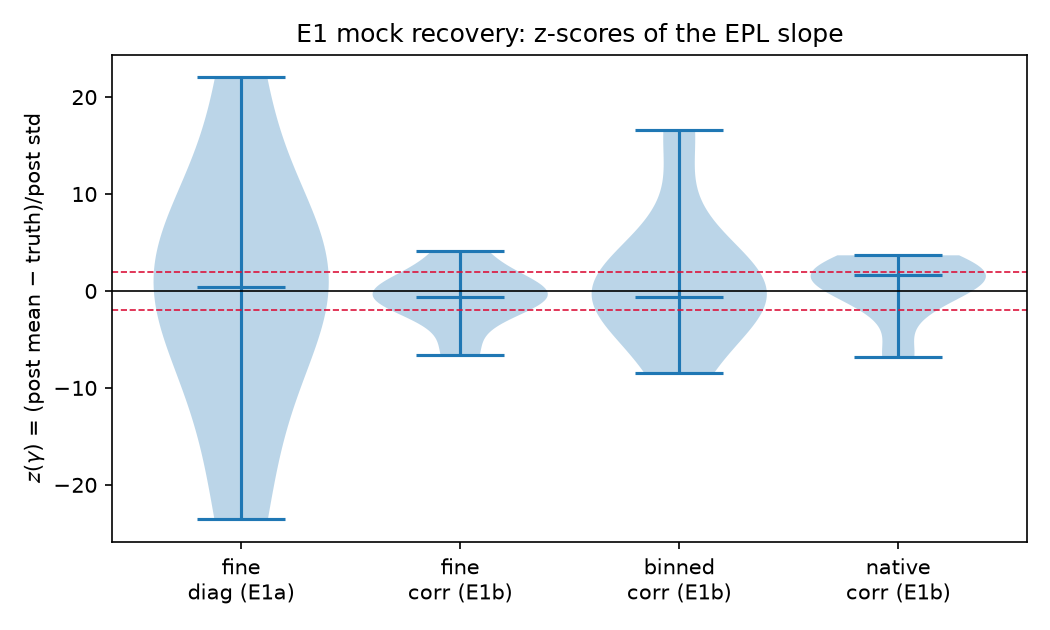
\includegraphics[width=0.82\textwidth]{../figs/e1_zscore_violins.png}
\caption{Recovered-slope $z$-score distributions across mocks, by product scale
and likelihood. The diagonal likelihood on drizzle-correlated fine mocks (the
E1a artifact) produces the broad, biased violin; the correlated likelihood
under the two-stage recipe centers each scale within the $|\bar z|<0.5$ band.
Source: \dfile{08\_pool\_e1.py}.}
\label{fig:e1violins}
\end{figure}

\begin{figure}[ht]
\centering
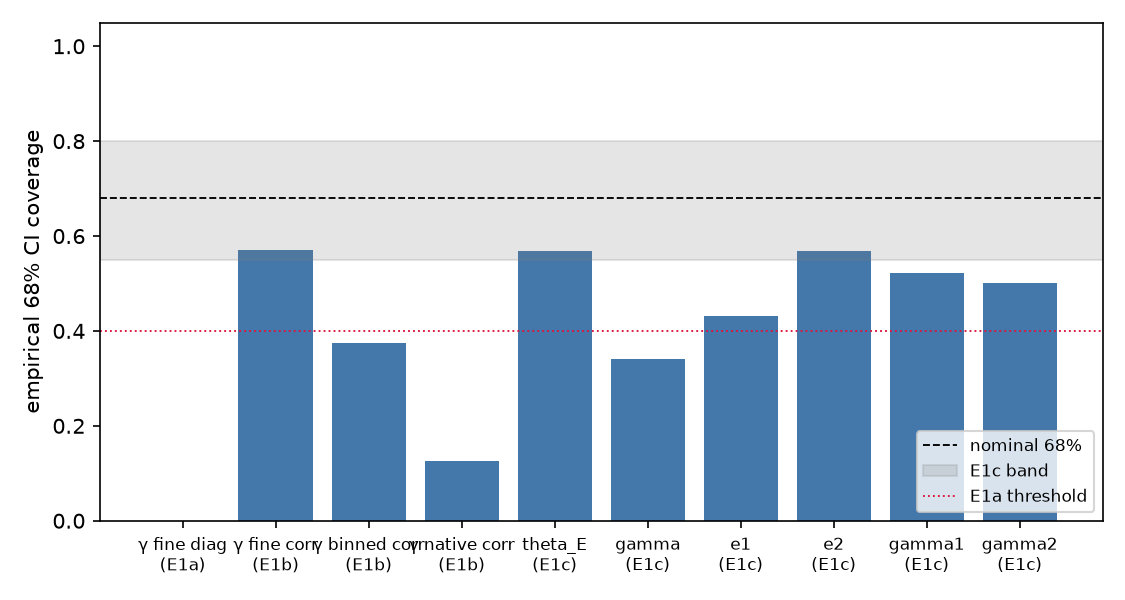
\includegraphics[width=0.49\textwidth]{../figs/e1_coverage.png}\hfill
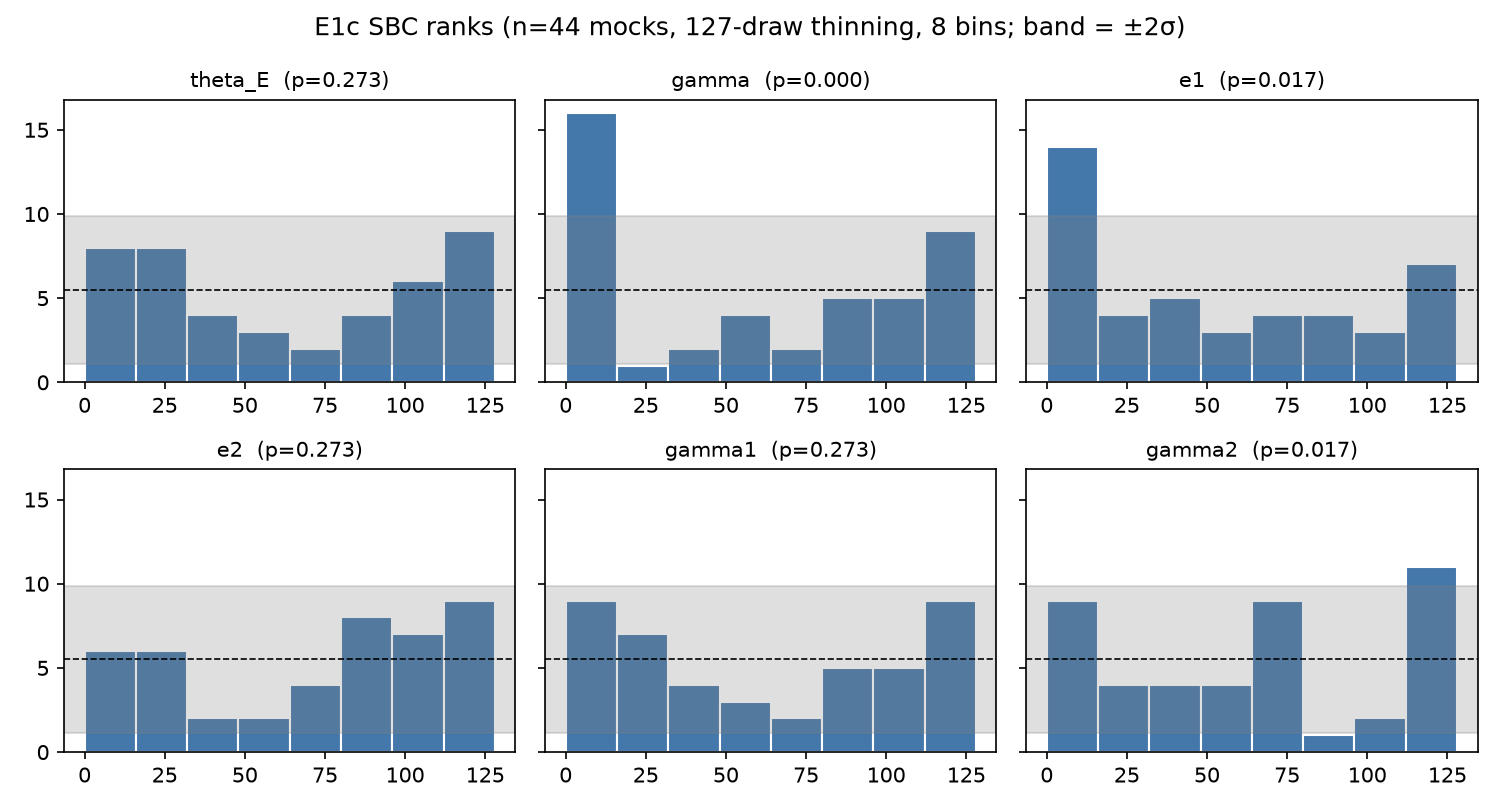
\includegraphics[width=0.49\textwidth]{../figs/e1_sbc_ranks.png}
\caption{Left: empirical $68\%$ coverage per parameter (healthy fits), with the
$[55,80]\%$ acceptance band. Right: SBC rank histograms; $\gammaEPL$ is uniform
on healthy fits, and the U-shape that flagged it over the full set is the
signature of under-mixed chains, not miscalibration (\S\ref{sec:twostage}).}
\label{fig:e1coverage}
\end{figure}

\begin{figure}[ht]
\centering
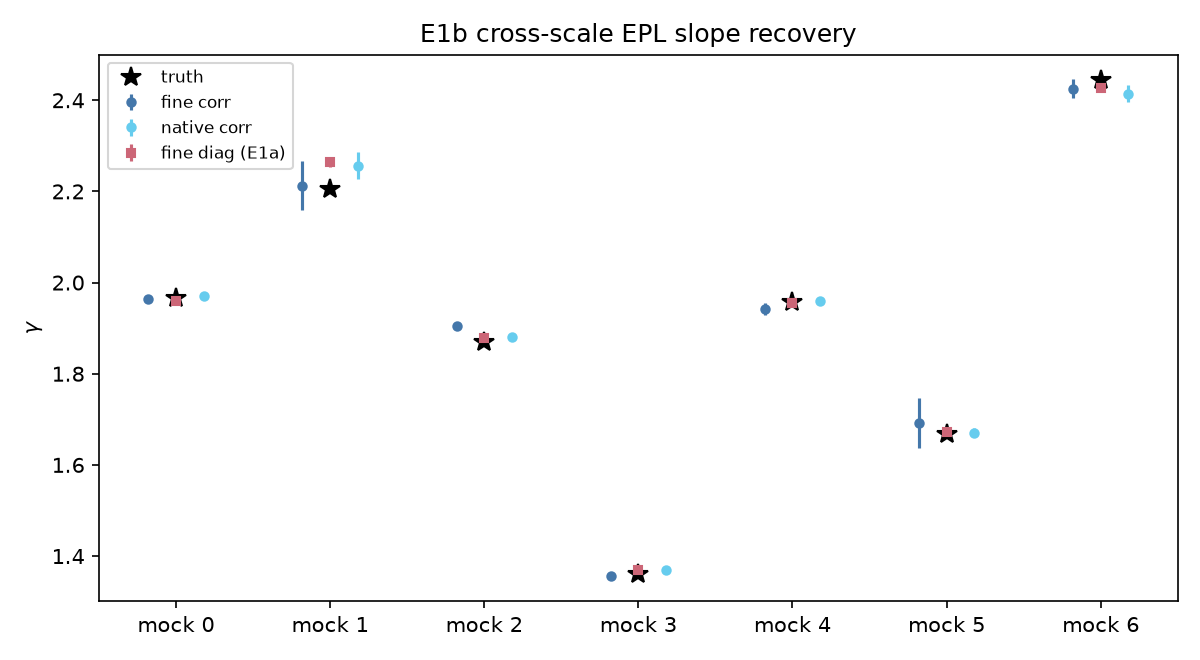
\includegraphics[width=0.82\textwidth]{../figs/e1_cross_scale.png}
\caption{Cross-scale slope agreement on mocks: fine versus native
$\gammaEPL$ under the correlated likelihood, with combined $1\sigma$ error
bars. Seven of eight pairs agree within $1\sigma_{\rm comb}$; the fine
posteriors are systematically wider (the characterized
$\sigma_{\rm fine}/\sigma_{\rm native}=2.45$ information cost, not a bias).}
\label{fig:e1crossscale}
\end{figure}

%%%%%%%%%%%%%%%%%%%%%%%%%%%%%%%%%%%%%%%%%%%%%%%%%%%%%%%%%%%%%%%%%%%%%%%%%%%%%%%
\section{Real-Data Cross-Scale Unification and the Bimodality Verdict}
\label{sec:realdata}
%%%%%%%%%%%%%%%%%%%%%%%%%%%%%%%%%%%%%%%%%%%%%%%%%%%%%%%%%%%%%%%%%%%%%%%%%%%%%%%

\noindent\emph{This section is gated on the P1c cross-scale run (Perlmutter,
$\le30$ A100-h, in progress). The frame, the pre-registered hypotheses, and the
figure slots are fixed here; only the verdict numbers remain.}
\todo{P1c: fill H1/H2/H3 verdicts, $\gammaEPL^{\rm fine}$(corr) vs the diagonal-native anchor 1.433, the money figure (Fig.~\ref{fig:money}), and the bimodality resolution table.}

\medskip
The correlated likelihood is applied to all three real products of \foundry\
under the two-stage PHMC recipe, with multi-basin starts, testing three
pre-registered hypotheses (both branches of each written down in advance; no
goalpost moves). The native fit uses the D3-adopted relaxed whitener; a
pre-registered amendment (recorded before any converged run) anchors H2/H3 on
the {\it diagonal}-native fit $\gammaEPL=1.433\,[1.400,1.469]$, because the
relaxed-whitener native correlated fit is likelihood-weak (information-limited
by pixel loss, the real-data analogue of the E1b width finding) and is
prior-pulled toward $\gammaEPL\approx2.0$; its width is reported separately as a
pixel-loss information-cost diagnostic. The money comparison is therefore
whether the correlated likelihood pulls the fine-product artifact
($\gammaEPL=2.585$ under the diagonal likelihood) back toward the trustworthy
native anchor.

\begin{description}
\item[H1 --- bimodality.] {\it Artifact branch:} under the correlated
likelihood the \dfile{v3}/\dfile{v3b} steep basin carries posterior mass
$<10\%$, or the corrected $\Delta\log\ell(\text{steep}-\text{low})\le0$ at the
basin MAPs $\Rightarrow$ the bimodality is a likelihood artifact.
{\it Survival branch (equally publishable):} the bimodality survives a
validated correlated likelihood $\Rightarrow$ it is a genuine or
PSF-systematic multimodality, and \dfile{v3b} becomes the flagship P2 target.
\todo{P1c: H1 verdict + steep-basin mass / corrected Delta-log-ell at basin MAPs.}
\item[H2 --- cross-scale unification.] $|\gammaEPL^{\rm fine}-\gammaEPL^{\rm
native}|$ and $|\gammaEPL^{\rm binned}-\gammaEPL^{\rm native}|<2\sigma_{\rm
comb}$ (anchor $\gammaEPL^{\rm native}(\mathrm{diag})=1.433\,[1.400,1.469]$);
the stronger form requires overlapping $68\%$ intervals.
\todo{P1c: H2 verdict + gamma at all three scales under the correlated likelihood.}
\item[H3 --- honesty.] $\sigma_\gamma(\text{fine, corr})\ge
\sigma_\gamma(\text{native, diag})/1.5$ (same photons must not manufacture
information). \todo{P1c: H3 verdict + sigma-gamma ratio.}
\end{description}

\gatedfigure{fig:money}{{\bf (Headline figure.)} Cross-scale slope of \foundry:
diagonal versus correlated likelihood at the fine, binned, and native scales,
with $68\%$ intervals and the diagonal-native anchor $1.433$ marked. The claim
under test is that the correlated likelihood collapses the diagonal
likelihood's scale-dependent slopes ($2.585$/$1.29$/$1.43$) onto a single
value.}{P1c: generate the diagonal-vs-correlated cross-scale slope figure once the converged real-data runs land.}

\gatedfigure{fig:bimodality}{The \dfile{v3b} binned $\gammaEPL$ posterior before
(diagonal) and after (correlated) --- the two disconnected basins under the
diagonal likelihood, and their fate under the correlated likelihood (H1). The
diagonal reference shows $45/3$ chains in the low/steep basins with zero
migrations.}{P1c: generate the v3b bimodality before/after panel from the converged multi-basin runs.}

%%%%%%%%%%%%%%%%%%%%%%%%%%%%%%%%%%%%%%%%%%%%%%%%%%%%%%%%%%%%%%%%%%%%%%%%%%%%%%%
\section{Sampler Benchmark Results}
\label{sec:benchmark}
%%%%%%%%%%%%%%%%%%%%%%%%%%%%%%%%%%%%%%%%%%%%%%%%%%%%%%%%%%%%%%%%%%%%%%%%%%%%%%%

The benchmark comprises $370$ evaluation cells (Track~A $345/351$, the six
omissions being pre-registered structured failures, plus $24$ Track~B cells),
consuming $202.4$ phoenix GPU-h and zero Perlmutter budget.\art{data/bench\_report.json}
The T0/T1 story is complete and settled below; the until-converged story on the
hardest real targets (T2 cond-$10^{14}$, T3 bimodal) is the A100 phase P2c and
is flagged as an open item where it appears. Figure~\ref{fig:benchmatrix} is the
full efficiency matrix.

\subsection{\nautilus\ dominates efficiency --- but is disqualified where it
matters most}

\nautilus\ \citep{lange2023nautilus} dominates sampling efficiency wherever it
applies: its median ESS/gradient beats the \gigalens\ baseline by
$2.6$--$307\times$ across the zoo (e.g.\ $180.7\times$ on the hard
\citet{gu2022gigalens} system 3, $307\times$ on system 11, $94\times$ on the
funnel, $114\times$ on the well-separated mixture), it returns the best
evidence estimates, and it recovers mixture modes (Table~\ref{tab:matrix}).
{\it But} it is {\it disqualified} on the condition-number-$10^{14}$ regime that
the real marginalized lens posterior actually occupies: on \dfile{t0\_illcond46}
its live-point shells collapse (fewer than eight equal-weight points in
$74$~minutes) and its evidence estimate errs by $\sim$$10^{7}$~nat. Its
reported ESS is moreover importance-weight ESS with a weak pseudo-$\Rhat$ on
exchangeable draws --- a semantics caveat we record rather than paper over: we
do not fail \nautilus\ on the $\Rhat$ criterion, but its mode-occupancy and
evidence carry its weight, and neither survives cond-$10^{14}$.

\subsection{At budget parity, no gradient method beats the baseline on T1}

The sharpest budget-matched result is negative and important: {\it under Track-A
budget parity, no gradient-based contender beats the \gigalens\ baseline (S0) on
the evaluation T1 systems.} The best gradient challenger, unadjusted MCLMC with
an SVI-diagonal metric, reaches at most $1.3\times$ the baseline ESS/gradient
(system 1) and a median below $1\times$; NUTS, tempered SMC, NeuTra, and the
GL-NT recipe are all well below parity on T1. Efficiency dominance on T1 belongs
to \nautilus\ alone --- and \nautilus\ is the sampler that fails the real
marginalization regime. The reliable-but-not-faster methods (S0, PT-HMC) and the
fast-but-fragile method (\nautilus) thus map onto different columns of the same
matrix, which is the benchmark's central lesson.

\subsection{Until converged, reliability inverts toward PT-HMC}

The Track-B (until-converged) ranking inverts the efficiency ranking.
Parallel-tempered HMC (\texttt{remc\_pt}) converges $5$ of $6$ hard T1 systems,
{\it including} system 6, where the baseline does not converge; it fails only
system 11 (where the baseline also fails). By contrast the baseline uniquely
{\it owns} the cond-$10^{14}$ regime: on \dfile{t0\_illcond46} S0 is the only
healthy gradient method ($\Rhat=1.00$) besides MCLMC ($\Rhat=1.04$), while
PT-HMC blows up ($\Rhat\sim10^{16}$ with its Track-A $\beta$-ladder), NUTS
reaches $\Rhat=3.76$, and NeuTra $\Rhat=5.72$.

\subsection{\flowmc\ fails structurally; GL-NT fails its own bars at Track-A
budget}

\flowmc\ \citep{wong2023flowmc} (version 0.4.5) is a {\it structural} failure on
lens posteriors, not a tuning miss: its scalar-MALA local step has no per-dim
preconditioning, so on the ill-conditioned $z$-space it holds $\Rhat=1.9$--$2.1$
across T1, converges $0/6$ Track-B systems even at $4\times$ budget, and {\it
inverts} the mixture on \dfile{t0\_mix22} (occupancy $0.13/0.87$ versus the true
$0.8/0.2$). This is a benchmark datum on the limits of flow-global-move sampling
without local preconditioning.

The ranked recipe bet, GL-NT, {\it fails its own recipe bars at Track-A budget}:
its T1-hard ESS/gradient is $0.03$--$0.05\times$ the baseline (target $\ge3\times$),
it regresses on easy targets, and its rank-normalized $\Rhat=1.4$--$2.0$ ---
flow-space ChEES is the weak stage. Its mode recovery is real but partial (it
clears the $0.05$ mode-weight bar only in float-64 on the separated mixture) and
never unique. GL-NT is therefore the lowest-priority P2c item: flow-space HMC
needs re-tuning or an A100 budget before any ``recipe'' claim is admissible; per
the pre-registered criteria, the current evidence supports a {\it benchmark}
paper, not a {\it recipe} paper.

\subsection{Multimodality: who recovers the modes}

On the two-component mixtures the baseline, NUTS, and NeuTra collapse to a
single mode ($1.000/0.000$ on \dfile{t0\_mix2}); \nautilus, tempered SMC,
\flowmc, and PT-HMC recover both. On the {\it harder} well-separated mixture
\dfile{t0\_mix22}, only PT-HMC clears the $<0.05$ mode-weight bar (median error
$0.031$), while \flowmc\ inverts the weights. Mode-recovery reliability and
sampling efficiency are, again, different axes: the efficient methods are not
the reliable mode-finders and vice versa.

\subsection{The freeze generalizes (no dev$\to$eval overfit)}

Table~\ref{tab:deveval} closes the protocol loop. The evaluation-to-development
ESS/gradient ratios are $\sim$$1.0$ for every contender (\nautilus\ $1.10$, MCLMC
$1.04$, \flowmc\ $1.03$, GL-NT $1.03$), i.e.\ frozen policies do {\it not}
overfit the development split; the persistently poor methods (\flowmc\ $\Rhat\approx
1.96$, GL-NT $\approx1.45$ on both splits) are poor structurally, not overfit.
The one method whose {\it dev} efficiency is optimistic is the baseline itself
(eval/dev $=0.31$): the guard-mandated schedule makes S0 the honest, stronger
variant, so the ``no gradient method beats the baseline'' result is if anything
conservative.

\begin{table}[ht]
\centering
\caption{Development-versus-evaluation generalization of the frozen policies
(median over cells; \dfile{data/bench\_report.json}). Ratios near $1.0$ certify
no dev$\to$eval overfit.}
\label{tab:deveval}
\begin{tabular}{lcccc}
\toprule
method & dev ESS/grad & eval ESS/grad & eval/dev & eval $\Rhat$ (med) \\
\midrule
\nautilus       & $3.8\!\times\!10^{-2}$ & $4.2\!\times\!10^{-2}$ & 1.10 & 1.001 \\
S0 baseline     & $7.9\!\times\!10^{-3}$ & $2.4\!\times\!10^{-3}$ & 0.31 & 1.022 \\
PT-HMC          & $2.1\!\times\!10^{-3}$ & $1.5\!\times\!10^{-3}$ & 0.69 & 1.004 \\
MCLMC           & $1.4\!\times\!10^{-3}$ & $1.5\!\times\!10^{-3}$ & 1.04 & 1.010 \\
tempered SMC    & $1.6\!\times\!10^{-4}$ & $2.1\!\times\!10^{-4}$ & 1.29 & --- \\
NeuTra          & $2.4\!\times\!10^{-4}$ & $2.2\!\times\!10^{-4}$ & 0.91 & 1.160 \\
NUTS            & $3.7\!\times\!10^{-5}$ & $8.0\!\times\!10^{-5}$ & 2.15 & 1.090 \\
GL-NT           & $7.4\!\times\!10^{-5}$ & $7.6\!\times\!10^{-5}$ & 1.03 & 1.453 \\
\flowmc         & $7.4\!\times\!10^{-5}$ & $7.6\!\times\!10^{-5}$ & 1.03 & 1.956 \\
\bottomrule
\end{tabular}
\end{table}

\begin{table}[ht]
\centering
\caption{Budget-matched efficiency (median-3-seed ESS/gradient relative to the
S0 baseline) on representative targets, with mode recovery on the mixtures.
\checkmark/$\times$ under ``modes'' = both mixture modes recovered within the
$0.10$ occupancy tolerance. Full matrix: Fig.~\ref{fig:benchmatrix},
\dfile{data/bench\_report.json}. T2/T3 rows are the P2c A100 phase.}
\label{tab:matrix}
\begin{tabular}{lccccc}
\toprule
 & \multicolumn{3}{c}{ESS/grad vs S0} & \multicolumn{2}{c}{modes} \\
\cmidrule(lr){2-4}\cmidrule(lr){5-6}
method & gu-sys3 (hard) & funnel10 & illcond46 & mix2 & mix22 \\
\midrule
\nautilus     & 180.7 & 94.4 & DQ (shells) & \checkmark & $\times$ \\
S0 baseline   & 1.00  & 1.00 & {\bf 1.00 (owns)} & $\times$ & $\times$ \\
PT-HMC        & 1.87  & 0.11 & blows up & \checkmark & {\bf\checkmark} \\
MCLMC         & 1.08  & 5.46 & 0.02 (healthy) & $\times$ & $\times$ \\
tempered SMC  & 0.85  & 3.38 & --- & \checkmark & $\times$ \\
NUTS          & 0.09  & 0.81 & $\Rhat\,3.8$ & $\times$ & $\times$ \\
NeuTra        & 0.56  & 0.67 & $\Rhat\,5.7$ & $\times$ & $\times$ \\
\flowmc       & 0.41  & 1.40 & $\Rhat\,2.2$ & \checkmark & inverts \\
GL-NT         & 0.26  & 0.28 & --- & $\times$ & $\times$ \\
\midrule
T2 (real 46d, cond-$10^{14}$) & \multicolumn{5}{c}{\todo{P2c: bj\_mclmc vs S0 until-converged on T2}} \\
T3 (real 74d, bimodal)        & \multicolumn{5}{c}{\todo{P2c: nautilus + remc\_pt (retuned ladder) + S0 on T3}} \\
\bottomrule
\end{tabular}
\end{table}

\begin{figure}[ht]
\centering
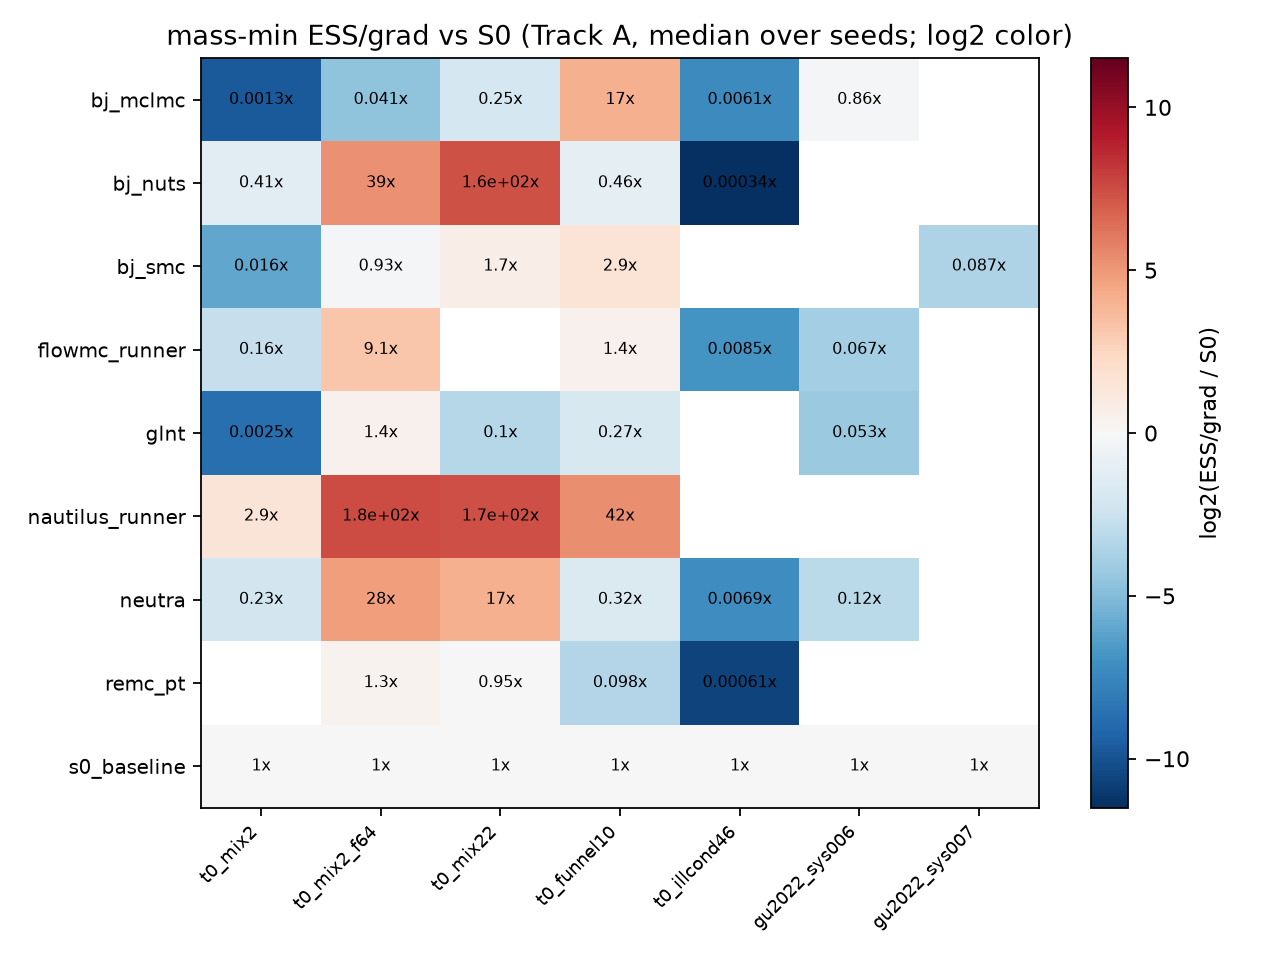
\includegraphics[width=0.99\textwidth]{../figs/bench_matrix.png}
\caption{The sampler $\times$ target efficiency matrix (Track~A, budget-matched,
median over three seeds): ESS/gradient relative to the \gigalens\ baseline, with
convergence ($\Rhat$) shading. \nautilus\ dominates the efficiency columns but
is disqualified on cond-$10^{14}$; the baseline and PT-HMC own reliability;
\flowmc\ and GL-NT are structurally weak on these geometries. Source:
\dfile{25\_pool\_benchmark.py}.}
\label{fig:benchmatrix}
\end{figure}

\paragraph{P2c plan (gated).} The A100 phase evaluates the two hardest real
targets until converged: T2 (cond-$10^{14}$) pits an SVI-diagonal-metric MCLMC
(an honest ``no hand-built mass matrix'' challenger) against the incumbent
baseline; T3 (bimodal) pits \nautilus\ (within-mode ESS and mode sensitivity,
not $\Rhat$) and a re-tuned-$\beta$-ladder PT-HMC against the S0 reference. GL-NT
is the drop-first item.
\todo{P2c: T2/T3 until-converged results, the T3 PT reference (>=100 beta=1 round trips, per-basin SMC evidence within 2 sigma), and the recipe-vs-benchmark verdict.}

%%%%%%%%%%%%%%%%%%%%%%%%%%%%%%%%%%%%%%%%%%%%%%%%%%%%%%%%%%%%%%%%%%%%%%%%%%%%%%%
\section{The CGL Recipe End-to-End, and Euclid Q1}
\label{sec:recipe}
%%%%%%%%%%%%%%%%%%%%%%%%%%%%%%%%%%%%%%%%%%%%%%%%%%%%%%%%%%%%%%%%%%%%%%%%%%%%%%%

\noindent\emph{This section is gated on P3 (end-to-end demonstration), which is
parked behind P1c and P2c.} The end-state combines the settled ingredients: the
correlated-noise likelihood (\S\ref{sec:methods1}) with the sampler that the
benchmark selects for the relevant regime (\S\ref{sec:benchmark}), applied to
\foundry\ end-to-end and to two--three Euclid Q1 grade-A lenses
\citep{euclidq1_slde_2025}, with \coolest-standard exports
\citep{coolest2023}.
\todo{P3: end-to-end CGL recipe on \foundry\ (correlated likelihood + selected sampler), the recipe-vs-benchmark determination against the README criteria, and 2--3 Euclid Q1 fits with theta-E vs published.}

\gatedfigure{fig:recipepanel}{End-to-end CGL recipe on \foundry: data, corrected
correlated-likelihood model, residual, and the unified cross-scale posterior,
with sampling diagnostics ($\Rhat$, ESS) at published compute
scale.}{P3: build the end-to-end recipe panel.}

\gatedfigure{fig:euclid}{Euclid Q1 comparison: CGL-recipe $\thetaE$ and
$\gammaEPL$ for 2--3 grade-A lenses against the published strong-lens
catalogue values.}{P3: build the Euclid Q1 comparison figure.}

%%%%%%%%%%%%%%%%%%%%%%%%%%%%%%%%%%%%%%%%%%%%%%%%%%%%%%%%%%%%%%%%%%%%%%%%%%%%%%%
\section{Discussion}
\label{sec:discussion}
%%%%%%%%%%%%%%%%%%%%%%%%%%%%%%%%%%%%%%%%%%%%%%%%%%%%%%%%%%%%%%%%%%%%%%%%%%%%%%%

The settled results already sharpen the field's picture on both axes. On the
likelihood axis, we have shown --- with known truth --- that ignoring drizzle
correlation is not a benign approximation: it biases the recovered slope at
$|z|\approx6$ and destroys coverage, and it does so even at native scale under
the real correlation kernel. The correlated likelihood removes that bias and
unifies the scales in mocks; whether it does so on the real system, and whether
it dissolves the \dfile{v3b} bimodality, is the pre-registered P1c fork
(\S\ref{sec:realdata}), both branches of which are publishable. The honest
standing caveat --- the fine posterior is {\it conservative} by a factor $2.45$
because near-singular drizzle covariances lose information at spectral zeros ---
is itself a useful result: it quantifies the price of correctness and motivates
the $\lambda$-sensitivity robustness scan.

On the inference axis, the benchmark's two-sided verdict is a caution against
single-number sampler comparisons. The most efficient sampler (\nautilus) is
disqualified precisely on the regime the real marginalized lens posterior
occupies; the most reliable until-converged sampler (PT-HMC) is not the most
efficient; and no gradient method beats the incumbent baseline at budget parity
on the standard mocks. That the ranked flow-assisted recipe (GL-NT) fails its
own bars at phoenix budget is a genuine finding, not a null result: it delimits
where transport-preconditioned HMC helps and where flow-space trajectory
adaptation is the bottleneck.

Two follow-on pillars are deliberately parked (out of scope, per the campaign's
written scope gate) and noted for completeness: a Gaussian-process / pixelated
source model (the natural successor to the shapelet source, and a stress test of
the correlated likelihood under a flexible source), and higher-order multipole
mass structure \citep{vandevyvere2022multipoles,powell2022multipoles}, whose
$\sim$$1\%$-level effects on \gammaEPL\ are of the same order as the
correlated-noise systematic quantified here. Both interact with the mass-sheet
degeneracy that limits time-delay cosmography \citep{tdcosmo4} and are the
subject of a planned P3 follow-on.

%%%%%%%%%%%%%%%%%%%%%%%%%%%%%%%%%%%%%%%%%%%%%%%%%%%%%%%%%%%%%%%%%%%%%%%%%%%%%%%
\section{Reproducibility}
\label{sec:repro}
%%%%%%%%%%%%%%%%%%%%%%%%%%%%%%%%%%%%%%%%%%%%%%%%%%%%%%%%%%%%%%%%%%%%%%%%%%%%%%%

\paragraph{Substrate and parity.} All experiments run against a vendored,
unpatched snapshot of the group production library (\texttt{gigalens-sean},
branch \texttt{multinode-2025}, ref \texttt{58ec9a7}) --- bit-identical to the
one the Foundry-I reproduction validated --- with every campaign modification in
a thin \texttt{cgl} package whose likelihood and marginalization take array-only
APIs (no \gigalens\ imports), so that any $\Delta\gammaEPL$ is attributable to
the likelihood change and not to the substrate. Parity against the validated
Foundry-I marginalization core passes all five pre-registered gates at machine
precision (Appendix~\ref{app:parity}).

\paragraph{Environment.} The pinned stack (identical core to the blessed
\gigalens\ venv: \texttt{jax}~0.6.2, \texttt{tensorflow-probability}~0.25.0,
\texttt{numpy}~2.4.6, \texttt{scipy}~1.17.1, \texttt{optax}~0.2.8,
\texttt{lenstronomy}~1.14.0, plus \texttt{blackjax}~1.3, \texttt{flowMC}~0.4.5,
\texttt{flowjax}~19.0.0, \texttt{nautilus-sampler}~1.0.6) is frozen to
$147$ packages and reproduced with zero resolver drift on both architectures
(aarch64 phoenix and Perlmutter x86-A100), the A100 parity re-verified fresh
(\S\ref{app:parity}). A single \texttt{constraints.txt} pins the sampler
dependencies that would otherwise silently upgrade \texttt{jax}.

\paragraph{Seven documented stack defects.} Reaching the settled state surfaced
seven reproducible issues in the \texttt{jax}~0.6.2 / TFP~0.25.0 sampler stack
(Table~\ref{tab:defects}); they are genuine findings, each with a workaround
carried in \texttt{cgl}. Two further correctness traps were caught and pinned:
an \textsc{arviz} axis-order bug that silently masked stuck chains (a
known-$\Rhat$-$2.07$ fit reported $1.00$ until the \texttt{(draw,chain)} axes
were corrected), and reversed per-parameter physical labels in the archived
\citet{gu2022gigalens} fits (block-contiguous, so aggregate mass sets are
unaffected; the zoo uses probed labels).

\begin{table}[ht]
\centering
\caption{The seven stack defects found and fixed during the campaign (detail in
\texttt{CAMPAIGN.md}). All are in the \texttt{jax}~0.6.2 / \texttt{jaxlib}~0.6.2
/ TFP~0.25.0 stack.}
\label{tab:defects}
\small
\begin{tabular}{p{0.36\textwidth}p{0.56\textwidth}}
\toprule
defect & workaround \\
\midrule
\#1 \texttt{chex}~0.1.92 silently upgrades \texttt{jax} 0.6.2$\to$0.10.2, breaking TFP & pin via \texttt{constraints.txt}; all installs pass \texttt{-c} \\
\#2 XLA \texttt{priority-fusion} livelocks fusing f64 \texttt{random.normal} with a reduction (MCLMC momentum refresh) & \texttt{XLA\_FLAGS=--xla\_disable\_hlo\_passes=priority-fusion}, set pre-import \\
\#3 \texttt{jaxlib} 0.6.2 triton GEMM aborts on tiny f32 dots (dim-2 SVI) on L4 & \texttt{--xla\_gpu\_enable\_triton\_gemm=false} (f64 immune) \\
\#4 priority-fusion livelock recurs in f32 (MCLMC tuner / NSF pipelines) & extend the flag to those adapters' processes \\
\#5 SMC particle-with-gradient memory ceiling $\sim$21\,MB/particle (1200 particles OOM a 24\,GiB L4) & cap particle count per device; frozen at 384/L4 \\
\#6 \nautilus\ jitted \texttt{log\_like} \texttt{TracerArrayConversion} on new batch sizes & batch padding + bijector-template probe \\
\#7 correlated-marg batched gradient ($28$ per-column convs under \texttt{vmap}) livelocks XLA compile & collapse to one depthwise/grouped conv; logp bit-identical, compiles in 13.8\,s \\
\bottomrule
\end{tabular}
\end{table}

\paragraph{Provenance and exports.} Every headline number in this report cites
its source JSON artifact (footnotes and inline \texttt{data/*.json}), and every
gate is a dated row in \texttt{CAMPAIGN.md}, which also carries the retracted
intermediate results verbatim (ledger discipline). The parity harness is
Appendix~\ref{app:parity}, the compute ledger Appendix~\ref{app:ledger}, the
zoo specification Appendix~\ref{app:zoo}, and the frozen sampler configurations
Appendix~\ref{app:configs}. The end-state products will be exported to the
code-independent \coolest\ standard \citep{coolest2023} in P3
(\S\ref{sec:recipe}).

%%%%%%%%%%%%%%%%%%%%%%%%%%%%%%%%%%%%%%%%%%%%%%%%%%%%%%%%%%%%%%%%%%%%%%%%%%%%%%%
\appendix

\section{Pre-Registered Verification Thresholds and Parity}
\label{sec:thresholds}
\label{app:parity}
%%%%%%%%%%%%%%%%%%%%%%%%%%%%%%%%%%%%%%%%%%%%%%%%%%%%%%%%%%%%%%%%%%%%%%%%%%%%%%%

Table~\ref{tab:thresholds} reproduces the pre-registered thresholds verbatim
from \texttt{README.md} \S Verification (frozen at P0, before any science ran).
Table~\ref{tab:parity} gives the measured parity-harness values.

\begin{table}[ht]
\centering
\caption{Pre-registered verification thresholds (verbatim, \texttt{README.md}
\S Verification). Goalposts fixed before any science run; changes require a
dated gate exception in \texttt{CAMPAIGN.md}.}
\label{tab:thresholds}
\small
\begin{tabular}{lll}
\toprule
gate & threshold & status \\
\midrule
A forward image        & $\max|\Delta|/\max|\mathrm{img}|\le10^{-12}$ (f64) & PASS \\
B log-posterior        & $|\Delta\log p|\le10^{-8}$ & PASS \\
C gradient             & relative $L_2\le10^{-8}$ & PASS \\
D diagonal limit       & corr.\ with $C=\mathrm{diag}$ equals diagonal stack $\le10^{-10}$ & PASS \\
E Occam term           & $-\tfrac12\log\det A$ vs numpy \texttt{slogdet} $\le10^{-10}$ & PASS \\
\midrule
whitener $\eop$        & $\le0.02$ & PASS \\
whitener MC whiteness  & $\mathrm{Var}(u)\in1\pm0.02$; $|$off-diag$|_{\le3}<0.01$ & PASS \\
whitener $|\Delta\log L|$ & $<0.1$ nat vs dense-$C$, $80^2/130^2$, 20 draws & PASS \\
kernel fit             & $\max|\rho_{\rm fit}-\rho_{\rm meas}|\le0.05$, model-subtracted & PASS \\
mock render            & $<0.05\sigma$ on every kept pixel & PASS \\
E1a artifact           & median $|z(\gammaEPL)|>2$ OR cov$_{68}<40\%$ & PASS \\
E1b recovery           & $|\bar z(\gammaEPL)|<0.5$/scale; cross-scale $\ge6/8$; width $\in[0.7,1.5]$ & PASS$^\ast$ \\
E1c SBC ($64$ mocks)   & rank $p>0.01$ each of $6$; cov$_{68}\in[55,80]\%$ & PASS$^\ast$ \\
E2 H1 bimodality       & steep mass $<10\%$ OR corrected $\Delta\log\ell\le0$ (both branches) & \todo{P1c} \\
E2 H2 cross-scale      & $|\Delta\gammaEPL|<2\sigma_{\rm comb}$; anchor $1.433\,[1.400,1.469]$ & \todo{P1c} \\
E2 H3 honesty          & $\sigma_\gamma(\text{fine})\ge\sigma_\gamma(\text{native})/1.5$ & \todo{P1c} \\
E3 robustness          & $\gammaEPL$-mean shift $<0.5\sigma$ across kernel variants & \todo{P3} \\
\midrule
P2 win criterion       & ESS/grad $\ge2\times$ AND $\Rhat<1.01$ AND modes $\pm10$ pts & applied \\
budget                 & Perlmutter commit $90$ A100-h, hard stop $100$, \texttt{deepsrch\_g} & on track \\
\bottomrule
\end{tabular}
\par\smallskip
{\footnotesize\textit{Note.} $^\ast$E1b width ratio and E1c full-set $\gammaEPL$
rank are met with the documented caveats of \S\ref{sec:mocks} (conservative-not-
biased width; healthy-fit restriction); the depth-controlled amendments are
recorded in \texttt{CAMPAIGN.md}.}
\end{table}

\begin{table}[ht]
\centering
\caption{Parity-harness measurements versus the validated Foundry-I
\texttt{\_hmc\_lib\_marg} core, at \texttt{map\_marg\_pd.npz} plus three seeded
perturbations and the \citet{gu2022gigalens} \texttt{system\_000} truth
(\dfile{data/parity\_report.json}).}
\label{tab:parity}
\begin{tabular}{llll}
\toprule
gate & threshold & achieved & note \\
\midrule
A forward image       & $10^{-12}$ & $6.2\times10^{-17}$ & f64, harness-rebuilt $m_{\rm det}$ \\
B log-posterior       & $10^{-8}$  & $0.0$ & worst of 4 points \\
C gradient rel-$L_2$  & $10^{-8}$  & $7.1\times10^{-17}$ & grad-norm $400.5806$ at $z_{\rm ref}$ \\
D diagonal limit      & $10^{-10}$ & $0.0$ & conv-whitener $=$ diagonal exactly \\
E Occam term          & $10^{-10}$ & $0.0$ & $\log\det A=323.229$, cond$(A)=1.4\times10^{4}$ \\
\midrule
(info) stored MAP logp & $10^{-5}$ & $6.5\times10^{-11}$ & pip-era A16 vs vendored L4 drift \\
(info) gu-2022 forward & $10^{-5}$ & $1.5\times10^{-6}$ & f32 stored render \\
\bottomrule
\end{tabular}
\end{table}

%%%%%%%%%%%%%%%%%%%%%%%%%%%%%%%%%%%%%%%%%%%%%%%%%%%%%%%%%%%%%%%%%%%%%%%%%%%%%%%
\section{Compute Ledger}
\label{app:ledger}
%%%%%%%%%%%%%%%%%%%%%%%%%%%%%%%%%%%%%%%%%%%%%%%%%%%%%%%%%%%%%%%%%%%%%%%%%%%%%%%

\noindent\emph{Partial --- the P1c/P2c/P3 Perlmutter rows are filled as they
charge.} All Perlmutter jobs charge account \texttt{deepsrch\_g}; the ledger row
is appended before results are read (\texttt{CAMPAIGN.md}). Committed
$\le90$ A100-h of the repo-wide allocation, hard stop $100$.

\begin{table}[ht]
\centering
\caption{Compute to the settled state. Phoenix is $8\times$A16~15\,GB $+
2\times$L4~23\,GB (budget-free, weekly-rolled); Perlmutter is $4\times$A100 per
node.}
\label{tab:ledger}
\begin{tabular}{llll}
\toprule
phase & platform & cost & note \\
\midrule
P0 staging + A100 parity  & Perlmutter & $1.2$ A100-h & parity A--E PASS both arch \\
P1c smoke (pre-flight)    & Perlmutter & $\le0.5$ A100-h & shared QOS \\
P1a--P1b (kernels, mocks, E1, diagnosis) & phoenix & $\sim$$165$ GPU-h & incl.\ $\sim$95 diagnosis \\
P2a--P2b (zoo, benchmark) & phoenix & $202.4$ GPU-h & $370$ cells \\
\midrule
P1c cross-scale (gated)   & Perlmutter & \todo{P1c: A100-h charged (<=30 committed)} & \\
P2c sampler matrix (gated)& Perlmutter & \todo{P2c: A100-h charged (<=45 committed)} & \\
P3 recipe + Euclid (gated)& Perlmutter & \todo{P3: A100-h charged (<=15 committed)} & \\
\bottomrule
\end{tabular}
\end{table}

%%%%%%%%%%%%%%%%%%%%%%%%%%%%%%%%%%%%%%%%%%%%%%%%%%%%%%%%%%%%%%%%%%%%%%%%%%%%%%%
\section{Posterior-Zoo Target Specifications}
\label{app:zoo}
%%%%%%%%%%%%%%%%%%%%%%%%%%%%%%%%%%%%%%%%%%%%%%%%%%%%%%%%%%%%%%%%%%%%%%%%%%%%%%%

The $19$ frozen targets (\dfile{data/zoo\_validation.json}) and their five
acceptance gates: (i) T1 zoo \texttt{log\_prob} bit-identical to direct
construction ($\max$ rel $0.0$); (ii) T2 \texttt{log\_prob} reproduces the
stored value to $\le10^{-8}$ ($\log p=-45840.984005998456$); (iii) T3 mass
bijector reproduction $0.0$ with basins measured $45$ low / $3$ steep
($\bar\gammaEPL^{\rm low}=1.294$, occupancy $0.9375/0.0625$, zero migrations);
(iv) T0 analytics recovered (logZ / mode occupancy, $\Rhat<1.001$); (v)
prior$+$like$=$prob consistency, worst relative $4.9\times10^{-8}$ (f32).

\begin{table}[ht]
\centering
\caption{The posterior zoo. dtype is the frozen evaluation precision; identity
tolerance is the adapter-fidelity assertion at three reference points.}
\label{tab:zoo}
\small
\begin{tabular}{lllp{0.40\textwidth}}
\toprule
target & tier & dtype & description \\
\midrule
\dfile{t0\_mix2} / \dfile{\_f64} & T0 & f32/f64 & two-component Gaussian mixture (0.8/0.2), analytic $Z$ + modes \\
\dfile{t0\_mix22}     & T0 & f32 & well-separated mixture (the hard mode-recovery target) \\
\dfile{t0\_funnel10}  & T0 & f32 & 10-d Neal funnel (varying curvature) \\
\dfile{t0\_illcond46} & T0 & f64 & 46-d ill-conditioned Gaussian, cond $\sim$$10^{14}$ (metric stress) \\
\dfile{gu2022\_sys000--011} & T1 & f32 & twelve \citet{gu2022gigalens} mock lens posteriors \\
\dfile{foundry\_marg46} & T2 & f64 & the $46$-d marginalized real posterior of \foundry\ (cond $10^{14}$) \\
\dfile{foundry\_v3b74}  & T3 & f32 & the $74$-d genuinely bimodal binned real posterior \\
(Euclid Q1 $\times$2--3) & T4 & --- & stub for the gated end-to-end phase (\S\ref{sec:recipe}) \\
\bottomrule
\end{tabular}
\end{table}

%%%%%%%%%%%%%%%%%%%%%%%%%%%%%%%%%%%%%%%%%%%%%%%%%%%%%%%%%%%%%%%%%%%%%%%%%%%%%%%
\section{Frozen Sampler Configurations}
\label{app:configs}
%%%%%%%%%%%%%%%%%%%%%%%%%%%%%%%%%%%%%%%%%%%%%%%%%%%%%%%%%%%%%%%%%%%%%%%%%%%%%%%

The frozen policies (\dfile{data/policies\_frozen.json},
\texttt{2026-07-06T22:08Z}; $\le8$ configs per method tuned on the dev split
only) are summarized in Table~\ref{tab:configs}; each carries a
content-addressed \texttt{sha\_config} and a rationale in the JSON. T0/T1 grad
budgets are $2\times10^5$/$1.5\times10^6$; Track~B scales these $\times4$ with
configuration pinned.

\begin{table}[ht]
\centering
\caption{Frozen T1 sampler configurations (representative fields;
\dfile{data/policies\_frozen.json}).}
\label{tab:configs}
\small
\begin{tabular}{lp{0.62\textwidth}}
\toprule
method & frozen configuration (key fields) \\
\midrule
S0 baseline & MAP$\to$SVI$\to$ChEES-HMC; $50$ chains $\times$($250$ burn $+750$ keep); guard-floored SVI \\
\blackjax\ NUTS & SVI start, target-accept $0.8$, tree-depth cap $2^6$ (bounds grad budget), diagonal mass \\
\blackjax\ MCLMC & unadjusted, tuner preconditioning, SVI-diagonal mass fallback for the cond-$10^{14}$ tuner collapse \\
\blackjax\ SMC & adaptive tempered, target-ESS $0.7$, $3$ MCMC steps, $5$ leapfrog, $1000$ particles \\
\flowmc & prior start, RQSpline ($4$ layers, $8$ bins, $64{\times}64$), scalar MALA step $0.6$, $32$ chains \\
\nautilus & $1000$ live, $4$ networks, $f_{\rm live}=0.01$, cap $=2\times$ grad budget (gradient-free) \\
PT-HMC (remc\_pt) & $6$ replicas, $\beta_{\min}=0.2$ (T1), $8$ leapfrog, SVI mass; T3 ladder to be re-tuned (P2c) \\
NeuTra & SVI-flow pullback ($6$ layers, $8$ knots) then ChEES-HMC in flow space \\
GL-NT & MAP$\to$SVI$\to$SMC anneal $\to$ NSF fit $\to$ flow-space ChEES-HMC (the recipe under test) \\
\bottomrule
\end{tabular}
\end{table}

%%%%%%%%%%%%%%%%%%%%%%%%%%%%%%%%%%%%%%%%%%%%%%%%%%%%%%%%%%%%%%%%%%%%%%%%%%%%%%%
\bibliographystyle{plainnat}
\bibliography{references}

\end{document}
